% Dokumentklassen s�ttes til memoir.
% Manual: http://ctan.org/tex-archive/macros/latex/contrib/memoir/memman.pdf
\documentclass[a4paper,oneside,article]{memoir}

\usepackage{pgf}
\usepackage{tikz}
\usepackage{pgfplots}
\usetikzlibrary{arrows,automata}
\usepackage{verbatim}
 
% Danske udtryk (fx figur og tabel) samt dansk orddeling og fonte med
% danske tegn. Hvis LaTeX brokker sig over �, � og � skal du udskifte
% "utf8" med "latin1" eller "applemac". 
\usepackage{inputenc}
\usepackage[danish]{babel}
\usepackage[T1]{fontenc}
 
% Matematisk udtryk, fede symboler, theoremer og fancy ting (fx k�debr�ker)
\usepackage{amsmath,amssymb}
\usepackage{bm}
\usepackage{amsthm}
%\usepackage{mathtools}
 
% Kodelisting. Husk at l�se manualen hvis du vil lave fancy ting.
% Manual: http://mirror.ctan.org/macros/latex/contrib/listings/listings.pdf
\usepackage{listings}
 
% Fancy ting med enheder og datatabeller. L�s manualen til pakken
% Manual: http://www.ctan.org/tex-archive/macros/latex/contrib/siunitx/siunitx.pdf
%\usepackage{siunitx}

% Inds�ttelse af grafik.
\usepackage{graphicx}
\usepackage{float}
\usepackage{caption}
\usepackage{subcaption}
 
% Reaktionsskemaer. L�s manualen for at se eksempler.
% Manual: http://www.ctan.org/tex-archive/macros/latex/contrib/mhchem/mhchem.pdf
%\usepackage[version=3]{mhchem}
%\usepackage[noend]{algpseudocode}
%\usepackage{algorithm}

\usepackage{xcolor,colortbl}

\usepackage{listings}

\definecolor{javared}{rgb}{0.6,0,0} % for strings
\definecolor{javagreen}{rgb}{0.25,0.5,0.35} % comments
\definecolor{javapurple}{rgb}{0.5,0,0.35} % keywords
\definecolor{javadocblue}{rgb}{0.25,0.35,0.75} % javadoc

\lstset{language=Java,
basicstyle=\small, %\ttfamily,
keywordstyle=\color{javapurple}\bfseries,
stringstyle=\color{javared},
commentstyle=\color{javagreen},
morecomment=[s][\color{javadocblue}]{/**}{*/},
numbers=left,
numberstyle=\tiny\color{black},
stepnumber=1,
numbersep=10pt,
tabsize=4,
showspaces=false,
showstringspaces=false}

\newcommand{\notimplies}{%
  \mathrel{{\ooalign{\hidewidth$\not\phantom{=}$\hidewidth\cr$\implies$}}}}

\begin{document}
    \title{Mutual Exclusion - Disposition}
    \author{Lukas Peter J�rgensen, 201206057, DA4
            }
    \maketitle
    
    \chapter{What is Mutex}
    \textbf{Requirements:}
    \begin{enumerate}
    \item Mutually exclusive access
    \item Starvation (Every process will get a chance to access the resource)
    \item Deadlock freedom
    \item Fairness (Every process has a right to access the resource)
    \end{enumerate}
    
    \chapter{Centralized}
    \begin{figure}[H]
		\centering
		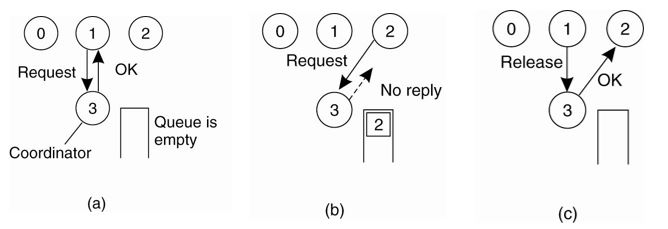
\includegraphics[width=\textwidth]{Media/MutexCentralized.jpg}
    \end{figure}
    \textbf{Mutual Exclusion?}\\
    Trivial.
    \textbf{Starvation?}\\
    Yes, trivial.
    \textbf{Deadlock freedom?}\\
    Yes, trivial.
    \textbf{Fairness?}\\
    Yes, since requests are granted in the order which they are recieved.
    
    \section*{Pros}
    \begin{itemize}
    \item Simple
    \item Easy to implement
    \item Low amount of messages to enter resource.
    \end{itemize}
    
    \section*{Cons}
    \begin{itemize}
    \item Single point of failure.
    \item Coordinator becomes bottleneck.
    \item Depending on implementation, it can be hard to distinquish dead coordinator from permission denied.
    \end{itemize}
    
    \chapter{Decentralized}
    Replicate resource $n$ times.\\
    When trying to access the resource, get a majority vote from $m > n/2$ coordinators.\\
    \\
    If a coordinator crashes, it's assumed that it forgets its vote but will recover quickly. It can handle up to $f$ failures where: $f<2m-n$
    
    \section*{Pros}
    \begin{itemize}
    \item Not as prone to failures as the centralized approach.
    \item Still relatively simple.
    \end{itemize}
    
    \section*{Cons}
    \begin{itemize}
    \item If a lot of processes want to access the resource, utilization drops. (Starvation)
    \end{itemize}
    
    \chapter{Distributed}
    Send out messages to all processes in the system, with a timestamp.\\
    3 cases to handle upon recieving such message:
    \begin{enumerate}
    \item Not accessing resource, and no interest: Send back "OK".
    \item Already has access, queue request and delay reply.
    \item Has an interest in accessing resource as well, compare timestamp. If incoming has the lowest timestamp, reply "OK". Else queue the request.
    \end{enumerate}
    
    \begin{figure}[H]
   		\centering
   		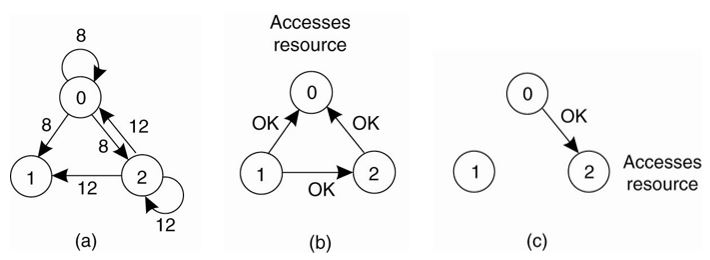
\includegraphics[width=\textwidth]{Media/MutexDistributed.jpg}
    \end{figure}
    
    \section*{Pros}
    \begin{itemize}
    \item No single point of failure exists.
    \end{itemize}
    
    \section*{Cons}
    \begin{itemize}
    \item Number of messages required per entry is $2(n-1)$.
    \item n points of failure.
    \item Dependent on information about the group of processes.
    \item All processes becomes possible bottlenecks.
    \end{itemize}
    
    \chapter{Token ring}
    Just send an "access token" through a ring of processes.\\
    Not much explanation needed.
    
    \section*{Pros}
    \begin{itemize}
    \item Fair, starvation free, deadlock free and ensures mutual exclusion.
    \item Efficient.
    \end{itemize}
    
    \section*{Cons}
    \textbf{What if the token is lost?}
    
    \chapter{Election}
    
    \chapter{Bully}
    \begin{enumerate}
    \item $P$ sends an \textit{ELECTION} message to all processes with higher numbers.
    \item If no one responds, $P$ wins the election and becomes coordinator.
    \item If one of the higher-ups answers, it takes over, $P$'s job is done.
    \end{enumerate}
    \begin{figure}[H]
     	\centering
     	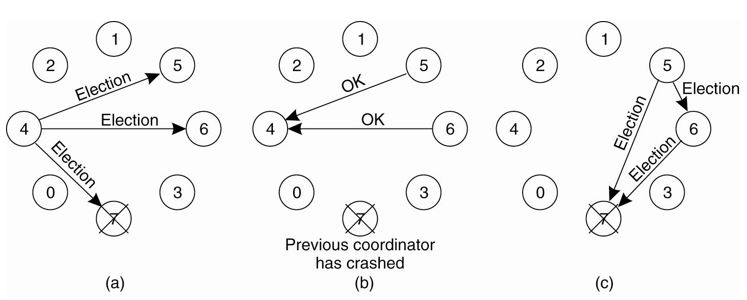
\includegraphics[width=\textwidth]{Media/Bully1.jpg}
    \end{figure}
    \begin{figure}[H]
    	\centering
    	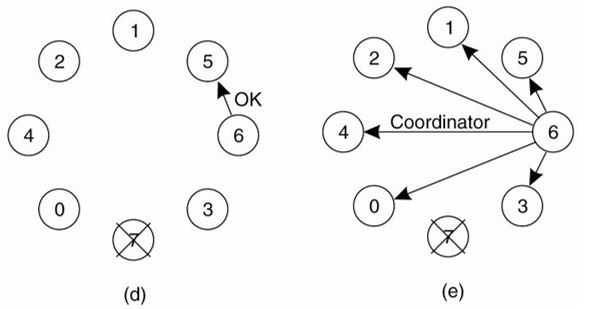
\includegraphics[width=\textwidth]{Media/Bully2.jpg}
    \end{figure}
    
    \chapter{Ring}
    Send out an "election" message and send it to the successor, each time reciever adds it's own number to the list, when initiater recieves its own election message, it will choose the highest number in the list and send out a "coordinator" message.
    \begin{figure}[H]
       	\centering
       	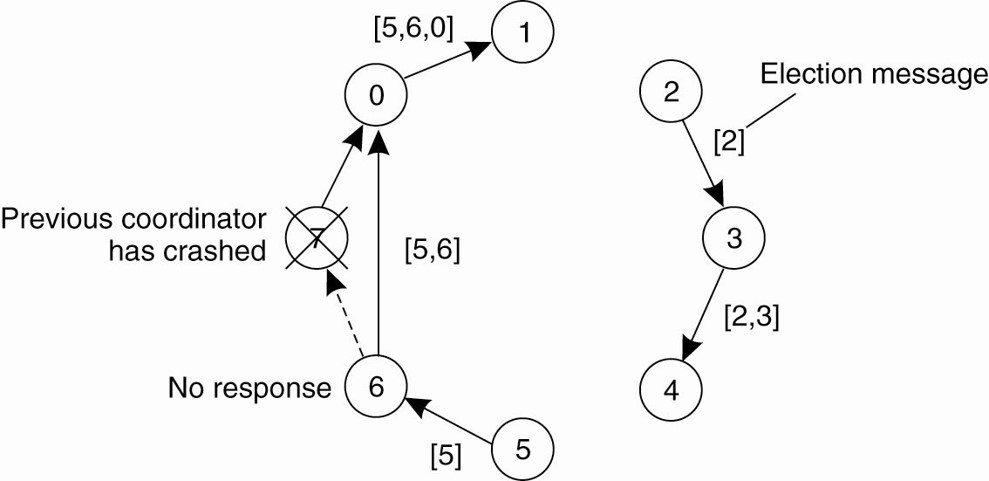
\includegraphics[width=\textwidth]{Media/RingElection.jpg}
    \end{figure}
    \textbf{Note:} Ours was a combination of ring and bully.
    
    \chapter{Election in wireless networks}
    When recieving an election message:
    \begin{enumerate}
    \item Assign sender as parent, send out election message to all neighbours except parent.
    \item If already participating in the election, respond immediately.
    \item When all neighbours have responded, return best candidate to parent.
    \item Use unique ID to determine most valid election.
    \end{enumerate}
    \begin{figure}[H]
       	\centering
       	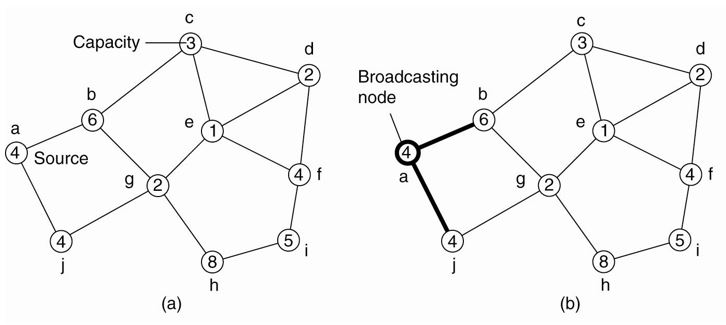
\includegraphics[width=\textwidth]{Media/WIFIElection1.jpg}
    \end{figure}
    \begin{figure}[H]
      	\centering
      	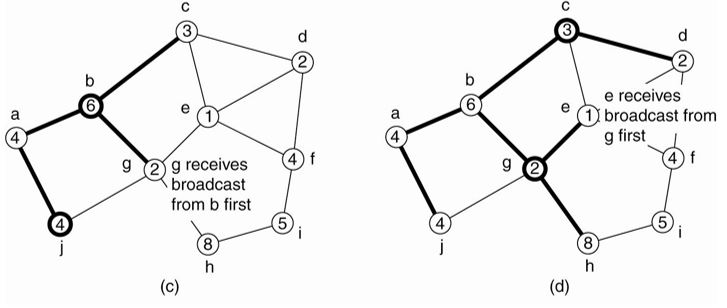
\includegraphics[width=\textwidth]{Media/WIFIElection2.jpg}
    \end{figure}
    \begin{figure}[H]
    	\centering
        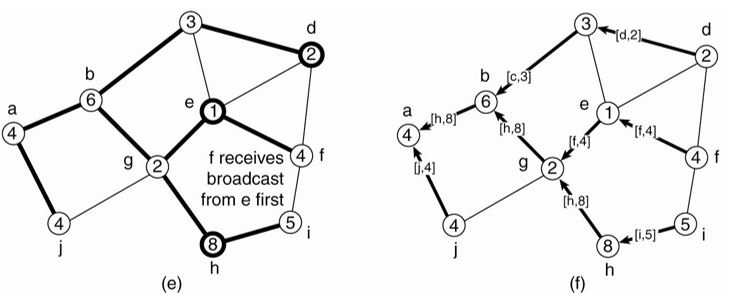
\includegraphics[width=\textwidth]{Media/WIFIElection3.jpg}
    \end{figure}
    
    \chapter{Large scale systems}
    \section*{Requirements for superpeer}
    \begin{enumerate}
    \item Normal nodes should have low-latency access to superpeers.
    \item Superpeers should be evenly distributed across the overlay network.
    \item Predefined portion of superpeers relative to the number of nodes.
    \item Each superpeer should not need to serve more than a fixed number of normal nodes.
    \end{enumerate}
    
    \section*{DHT}
    Assume we want $L$ leaders in $m$-bit Chord DHT.\\
    Use the $k=\lceil log_2(L) \rceil$ most significant bits.\\
    The leader for $p$ is $lookup(p \& 1^k000)$\\
    Each super peer is then responsible for an expected $\frac{2^k}{2^m}N nodes$.
    
\end{document}